\subsubsubsubsection{District}
\begin{figure}[h]
\centering
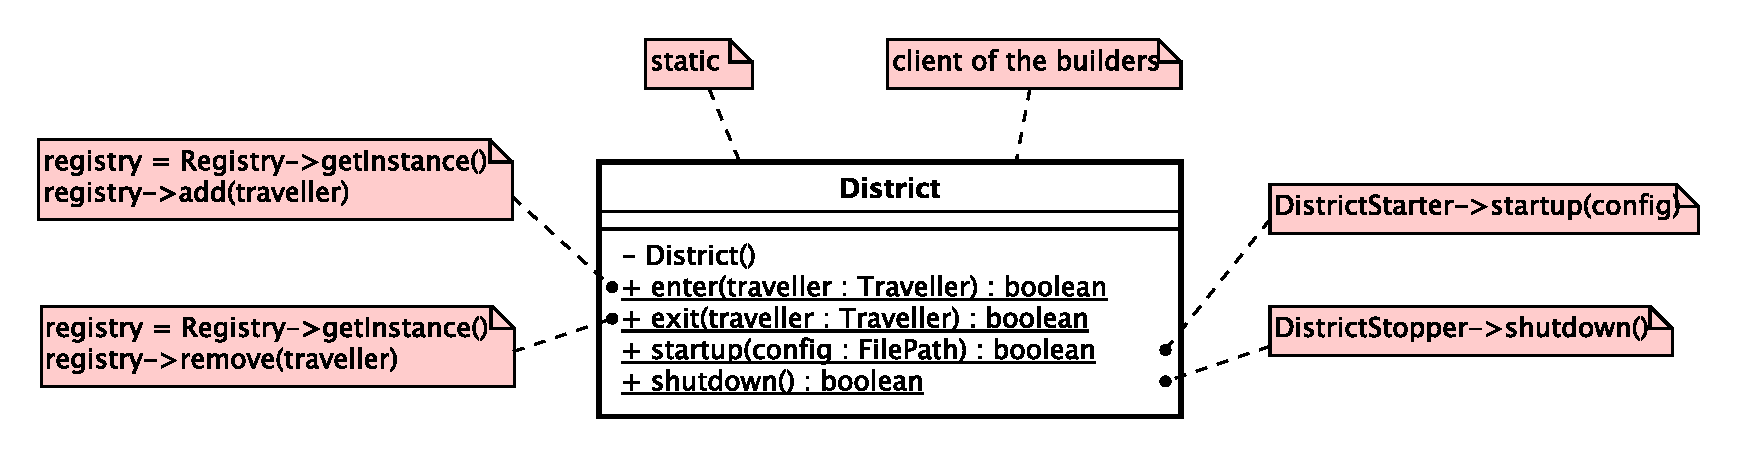
\includegraphics[scale=0.6,keepaspectratio]{images/solution/app/backend/district.eps}
\caption{\pReactive::District}
\label{fig:sd-app-district}
\end{figure}
\FloatBarrier
\begin{itemize}
  \item \textbf{\descr} \\
  It represents the master entity of the application layer.
  It is a static class because it is composed of only static methods.
  \item \textbf{\ops}
  \begin{itemize}
    \item \texttt{District()} \\
    Private and unique constructor because the class provides only static methods 
    so there are no reasons a client creates instances of it.
    \item[+] \texttt{\underline{enter(traveller: Traveller) : boolean}} \\
    Notifies the district to add a new traveller to the population.
    Returns true if the process completes neatly, false otherwise.
    \item[+] \texttt{\underline{exit(traveller: Traveller) : boolean}} \\
    Notifies the district to pass a traveller from the roadMap to the 
    application layer interface which communicates to the middleware layer.
    Returns true if the process completes neatly, false otherwise.
    \item[+] \texttt{\underline{startup(config: FilePath) : boolean}} \\
    Delegate the creation and boots all the entities of the district
    to \texttt{DistrictStarter}.
    Returns true if the process completes neatly, false otherwise.
    \item[+] \texttt{\underline{shutdown() : boolean}} \\
    Delegates the termination of the district
    to \texttt{DistrictStopper}.
    Returns true if the process completes neatly, false otherwise.
  \end{itemize}
\end{itemize} 
